\section{Arquitectura y Mecanismos de Seguridad}
\label{sec:seguridad_sistema}

La seguridad informática en esta página web no consiste en intentar lograr una protección absoluta al 100\% (lo cual es técnicamente imposible), sino en gestionar la incertidumbre de forma inteligente, preventiva y ordenada para cuidar lo que más importa \parencite{ferraiolo2007}. En una plataforma de seguimiento de tesis dentro de la Facultad de Ciencias de la Computación (FCC) de la BUAP se concentra información sensible de la comunidad: nombres oficiales, números telefónicos, historiales académicos, notas de asesoría y los borradores originales de investigación de los alumnos antes de su examen de grado.

Si el sistema careciera de candados estrictos, un usuario malintencionado o curioso podría intentar adivinar contraseñas, inventarse cuentas de profesor para aprobar trabajos sin autorización, alterar los acuerdos de las minutas o subir programas dañinos disfrazados de documentos escolares.

Por esta razón, la seguridad de la plataforma se diseñó bajo un \textbf{esquema integral de protección por capas}: la infraestructura de red cifra las comunicaciones, el framework Django filtra cada orden antes de tocar el servidor, y la base de datos MySQL resguarda la información aislada con permisos mínimos y consultas parametrizadas.

\subsection{Elementos que Requieren Protección y Clasificación de Datos}
\label{subsec:elementos_proteger}

Para cuidar la plataforma de forma metódica, los activos que maneja el sistema se agruparon en tres categorías principales:

\begin{enumerate}
    \item \textbf{Capa de Datos:} Contraseñas protegidas, correos institucionales, matrículas escolares, números de teléfono, archivos PDF de los borradores de tesis, minutas con compromisos calendarizados y registros de auditoría sobre inactividad.
    \item \textbf{Capa de Software:} El código desarrollado en Django y Python, los validadores de archivos en \texttt{validators.py}, el servidor web Nginx y el motor de base de datos MySQL (\texttt{tesina\_db}).
    \item \textbf{Capa de Infraestructura:} El servidor institucional donde corre la aplicación web, los volúmenes de almacenamiento en disco para los archivos multimedia (\texttt{media/}) y los equipos personales desde donde ingresan estudiantes y docentes.
\end{enumerate}

En México, la Ley Federal de Protección de Datos Personales en Posesión de los Particulares (LFPDPPP) y los reglamentos escolares establecen que cada persona es dueña de su información personal. En el Cuadro~\ref{tab:clasificacion_seguridad} se detalla la clasificación de estos datos dentro del sistema y los motivos obligatorios para su resguardo.

\begin{table}[H]
\centering
\small
\singlespacing
\caption{Clasificación de la información del sistema y justificación de protección.}
\label{tab:clasificacion_seguridad}
\begin{tabular}{p{3.6cm} p{5.0cm} p{6.8cm}}
\toprule
\textbf{Categoría de Dato} & \textbf{Datos dentro del Sistema} & \textbf{Motivo Escolar y Legal de Protección} \\
\midrule
Datos de Identificación Personal & 
Nombre completo, matrícula, correo institucional y número de teléfono. & 
Permiten identificar directamente a los miembros de la comunidad. Su filtración expondría a los usuarios a fraudes, robo de identidad o suplantación en los accesos. \\
\addlinespace
Historial Académico y Desempeño & 
Revisiones del asesor, historial de entregas, reportes de inactividad y estado de la tesis. & 
Información confidencial de la trayectoria escolar del alumno; nadie ajeno a su comité de titulación o a la coordinación debe enterarse de su avance. \\
\addlinespace
Propiedad Intelectual y Contenido & 
Archivos PDF de borradores, protocolos de investigación y acuerdos de minutas. & 
Contienen ideas y desarrollos tecnológicos originales antes de su publicación o examen profesional. Deben blindarse contra plagios o copias no autorizadas. \\
\bottomrule
\end{tabular}
\end{table}

\noindent \textbf{Respeto a los Derechos ARCO:} En apego a la privacidad de la comunidad académica, los datos recopilados en el sistema son de uso estrictamente escolar y no se comparten con terceros ajenos a la facultad. Cualquier estudiante o profesor puede solicitar el Acceso, Rectificación (corregir teléfonos o datos inexactos), Cancelación u Oposición respecto a su información mediante solicitud formal dirigida a la Coordinación Académica.

\subsection{Evaluación y Matriz de Riesgos (P x I)}
\label{subsec:evaluacion_riesgos}

Para decidir qué defensas técnicas debían programarse primero, no se actuó por suposiciones; se aplicó una matriz de riesgos basada en la probabilidad de que una amenaza suceda multiplicada por el impacto o daño que causaría en la facultad \parencite{ferraiolo2007}:
\begin{equation}
\text{Nivel de Riesgo} = \text{Probabilidad } (P) \times \text{Impacto } (I)
\end{equation}

Las escalas de evaluación se definieron bajo los siguientes criterios:
\begin{itemize}
    \item \textbf{Escala de Probabilidad ($P$):} 1 = Baja (muy difícil que ocurra), 2 = Media (podría pasar en algún momento), 3 = Alta (es muy probable que suceda si no se ponen candados).
    \item \textbf{Escala de Impacto ($I$):} 1 = Bajo (daño menor fácil de contener), 2 = Moderado (daño a la reputación interna o llamado de atención), 3 = Alto (violación de la LFPDPPP, multas o fuga de datos sensibles), 4 = Crítico (pérdida irreparable de datos, daño legal o suspensión de trámites).
\end{itemize}

En el Cuadro~\ref{tab:matriz_riesgos_sistema} se presenta la evaluación formal de los cuatro escenarios de riesgo identificados para el proyecto, junto con su nivel y el tratamiento implementado.

\begin{table}[H]
\centering
\small
\singlespacing
\caption{Matriz de riesgos de seguridad y controles de mitigación implementados.}
\label{tab:matriz_riesgos_sistema}
\begin{tabular}{c p{5.3cm} c c c c p{2.8cm}}
\toprule
\textbf{ID} & \textbf{Escenario de Riesgo} & \textbf{P} & \textbf{I} & \textbf{Nivel} & \textbf{Prioridad} & \textbf{Tratamiento} \\
\midrule
\textbf{R-01} & 
Fuga masiva de datos personales o expedientes por fallas en listas de acceso de red. & 
3 & 4 & 12 & \textbf{EXTREMA} & Mitigar de forma inmediata. \\
\addlinespace
\textbf{R-03} & 
Abuso de privilegios: un usuario con cuenta intenta espiar datos confidenciales ajenos (IDOR). & 
2 & 3 & 6 & \textbf{ALTA} & Mitigar y monitorear permanentemente. \\
\addlinespace
\textbf{R-02} & 
Acceso accidental a carpetas o funciones sin datos sensibles por un error de navegación. & 
2 & 2 & 4 & \textbf{MEDIA} & Mitigar y aceptar el riesgo residual. \\
\addlinespace
\textbf{R-04} & 
Ataques externos dirigidos a vulnerar la base de datos MySQL o infectar el servidor. & 
1 & 4 & 4 & \textbf{MEDIA} & Mitigar y transferir con respaldos externos. \\
\bottomrule
\end{tabular}
\end{table}

\noindent \textbf{Priorización y Análisis de las Defensas:}
\begin{enumerate}
    \item \textbf{Atención inmediata al riesgo R-01 (Nivel Extremo):} Es el peligro más crítico del proyecto porque combina una alta probabilidad con un impacto legal y escolar grave. Para eliminarlo, la página prohíbe el tráfico sin cifrar, utiliza cookies seguras con directivas \texttt{HttpOnly} y aísla la base de datos MySQL para que solo reciba peticiones locales del servidor web.
    \item \textbf{Control estricto contra el abuso de privilegios R-03 (Nivel Alto):} Ocurre cuando una persona con cuenta válida intenta cambiar números en la barra de direcciones para ver tesis ajenas. Se neutraliza aplicando el principio de mínimo privilegio: los asesores solo ven a sus propios alumnos y las consultas del backend quedan estrictamente amarradas a la sesión del usuario conectado (\texttt{request.user}).
    \item \textbf{Defensas operativas para riesgos medios R-02 y R-04:} Corresponden a descuidos de navegación y ataques automáticos desde internet. Se resuelven manteniendo activos los filtros contra falsificación de formularios (CSRF), la parametrización de consultas del ORM de Django y respaldos periódicos de la base de datos y la carpeta de medios.
\end{enumerate}

\subsection{Políticas de Ciberseguridad del Sistema}
\label{subsec:politicas_seguridad}

Las defensas técnicas requieren complementarse con reglas de conducta institucional claras para alumnos, asesores y coordinadores. En el Cuadro~\ref{tab:politicas_seguridad} se establecen cinco políticas obligatorias de ciberseguridad para la plataforma, distinguiendo con claridad entre una acción no intencional (negligencia o descuido) y una acción intencional (dolo o trampa).

\begin{table}[H]
\centering
\scriptsize
\singlespacing
\caption{Políticas de ciberseguridad, motivos y régimen de penalizaciones institucionales.}
\label{tab:politicas_seguridad}
\begin{tabular}{p{0.4cm} p{3.2cm} p{3.4cm} p{3.8cm} p{4.0cm}}
\toprule
\textbf{Nº} & \textbf{Regla o Política} & \textbf{Justificación Escolar} & \textbf{Sanción: Negligencia (Sin dolo)} & \textbf{Sanción: Dolo (Intencional)} \\
\midrule
1 & 
Uso obligatorio de contraseñas complejas (mínimo 10 caracteres combinando letras y números). & 
Reduce intentos de acceso no autorizado y ataques de adivinación de claves en el inicio de sesión. & 
Aviso automático del sistema y restablecimiento forzoso de contraseña en el siguiente ingreso. & 
Suspensión temporal del acceso y citatorio formal ante la Coordinación Académica. \\
\addlinespace
2 & 
Prohibición estricta de compartir cuentas, contraseñas o enlaces de sesión con terceros. & 
Garantiza la trazabilidad: cada avance en PDF o minuta debe pertenecer a su autor legítimo. & 
Amonestación por correo electrónico institucional y cambio forzoso de clave de acceso. & 
Bloqueo definitivo del acceso digital y reporte formal en el expediente escolar del usuario. \\
\addlinespace
3 & 
Carga exclusiva de avances en formato PDF legítimo y libre de contenido ejecutable. & 
Evita el ingreso de programas malignos, scripts o virus al disco duro del servidor escolar. & 
Rechazo automático del documento por el sistema y notificación con guía para exportar a PDF. & 
Cancelación del derecho de entrega en el periodo vigente y turnado al Consejo de Posgrado. \\
\addlinespace
4 & 
Respeto a la privacidad: prohibido alterar parámetros en la URL para consultar tesis ajenas. & 
Protege el derecho a la confidencialidad de las investigaciones y los historiales de posgrado. & 
Bloqueo de la petición (Error 403) y registro preventivo del incidente en la bitácora técnica. & 
Baja temporal del sistema de titulación y apertura de investigación por falta grave a la ética. \\
\addlinespace
5 & 
Cierre de sesión obligatorio al utilizar computadoras públicas o de la facultad. & 
Impide que una persona que utilice el equipo después suplante la identidad del estudiante. & 
Cierre automático de la sesión por el servidor tras un periodo de inactividad programado. & 
Amonestación por escrito y supervisión presencial obligatoria para trámites posteriores. \\
\bottomrule
\end{tabular}
\end{table}

\subsection{Filtrado de Peticiones y Seguridad del Servidor}
\label{subsec:seguridad_servidor_flujo}

Cada vez que un usuario hace clic en un botón, llena un formulario o sube un documento, su navegador web envía un mensaje por internet llamado petición. Para que una orden tramposa o dañina no pueda comprometer la plataforma, la petición tiene que cruzar tres filtros de seguridad obligatorios antes de poder tocar los datos.

En la Figura~\ref{fig:seguridad_pdf} se muestra cómo viaja la petición de izquierda a derecha a través de estas barreras defensivas:

\begin{figure}[H]
    \centering
    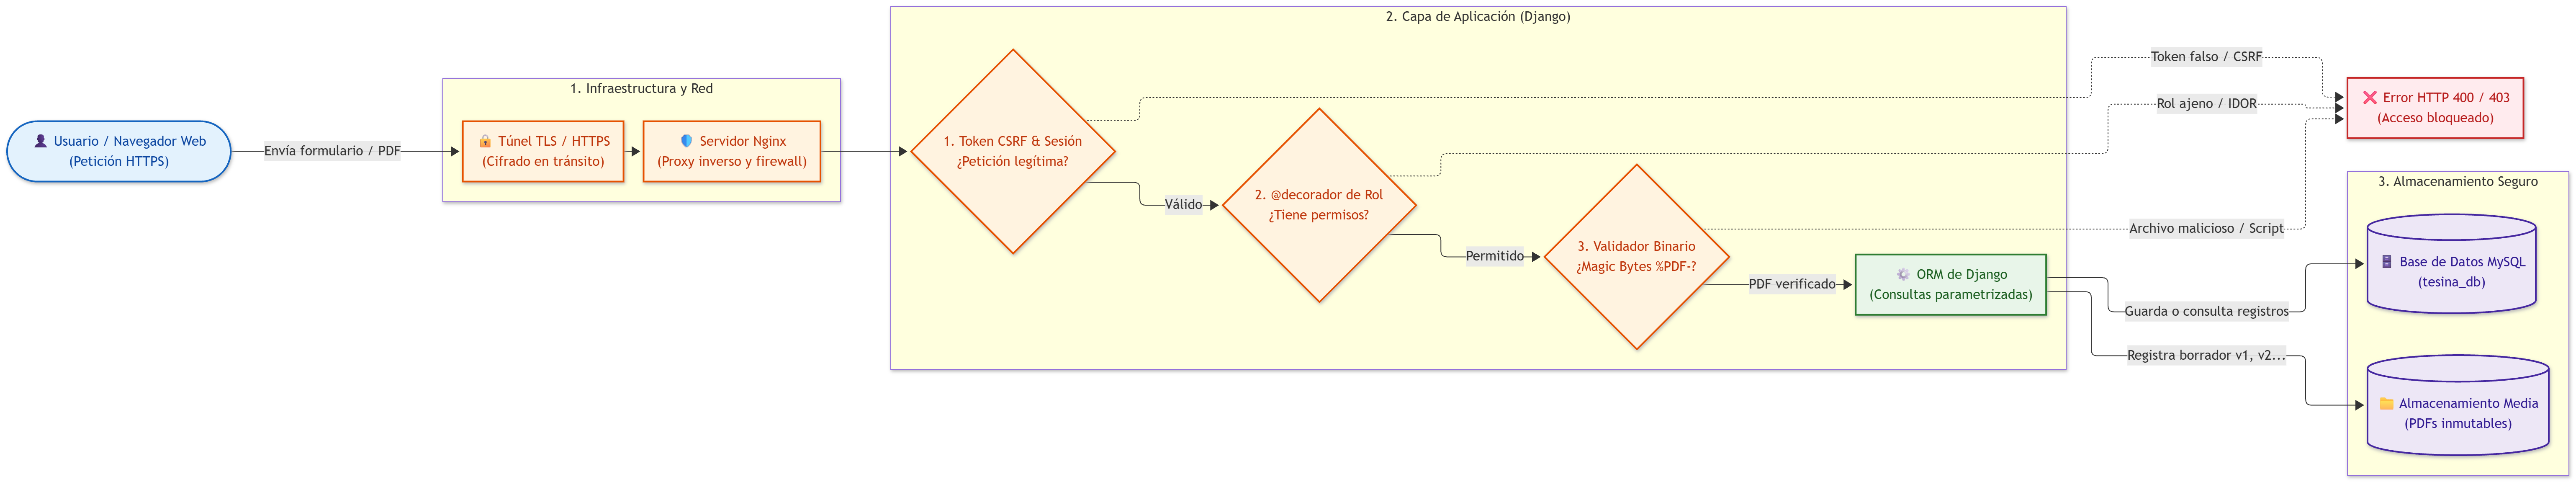
\includegraphics[width=\linewidth]{assets/seguridad/seguridad_pdf.png}
    \caption{Flujo horizontal de seguridad y filtros que debe superar cada petición en el servidor.}
    \label{fig:seguridad_pdf}
\end{figure}

\begin{enumerate}
    \item \textbf{Capa de Infraestructura y Red:} El usuario se conecta mediante un túnel seguro con protocolo HTTPS y cifrado TLS 1.3, lo que impide que alguien conectado a la misma red Wi-Fi de la facultad pueda espiar sus contraseñas o documentos. Al llegar al servidor, el programa Nginx actúa como guardia de entrada, canalizando únicamente el tráfico auténtico hacia el sistema.
    \item \textbf{Capa de Aplicación (Filtros en Django):} Aquí la plataforma realiza tres comprobaciones consecutivas:
    \begin{itemize}
        \item \textit{Token CSRF y Sesión:} Comprueba que la orden venga realmente de la ventana abierta por el alumno y no de una página falsa en internet.
        \item \textit{Decorador de Rol:} Revisa si la cuenta tiene el permiso correspondiente (por ejemplo, impidiendo que un alumno entre al panel del coordinador).
        \item \textit{Validador Binario:} Si la persona adjuntó un documento, examina que sea un PDF auténtico y no un script dañino.
    \end{itemize}
    Si alguna de estas comprobaciones falla, el sistema frena la petición de golpe y arroja un error de bloqueo (HTTP 400 o 403), sin tocar jamás la información.
    \item \textbf{Almacenamiento Seguro (ORM y MySQL):} Solo si la petición superó limpiamente todas las aduanas, el ORM de Django ejecuta órdenes ordenadas y guarda los registros en MySQL (\texttt{tesina\_db}) o almacena el archivo en la carpeta protegida de entregas.
\end{enumerate}

\subsection{Protección de Contraseñas mediante Cifrado Hash (Soporte al CU01)}
\label{subsec:seguridad_hasheo}

Una de las reglas más importantes en la página web es que \textbf{las contraseñas nunca se guardan tal como se escriben}. Si una persona escribe \texttt{Password123}, esa palabra jamás se almacena en texto plano dentro de la base de datos. Si alguien lograra abrir la tabla de usuarios, únicamente encontraría códigos largos, revueltos e imposibles de leer.

En la Figura~\ref{fig:seguridad_contrasena} se explica cómo funciona este proceso mediante una función matemática de una sola vía (algoritmo PBKDF2 con SHA-256 propio de Django):

\begin{figure}[H]
    \centering
    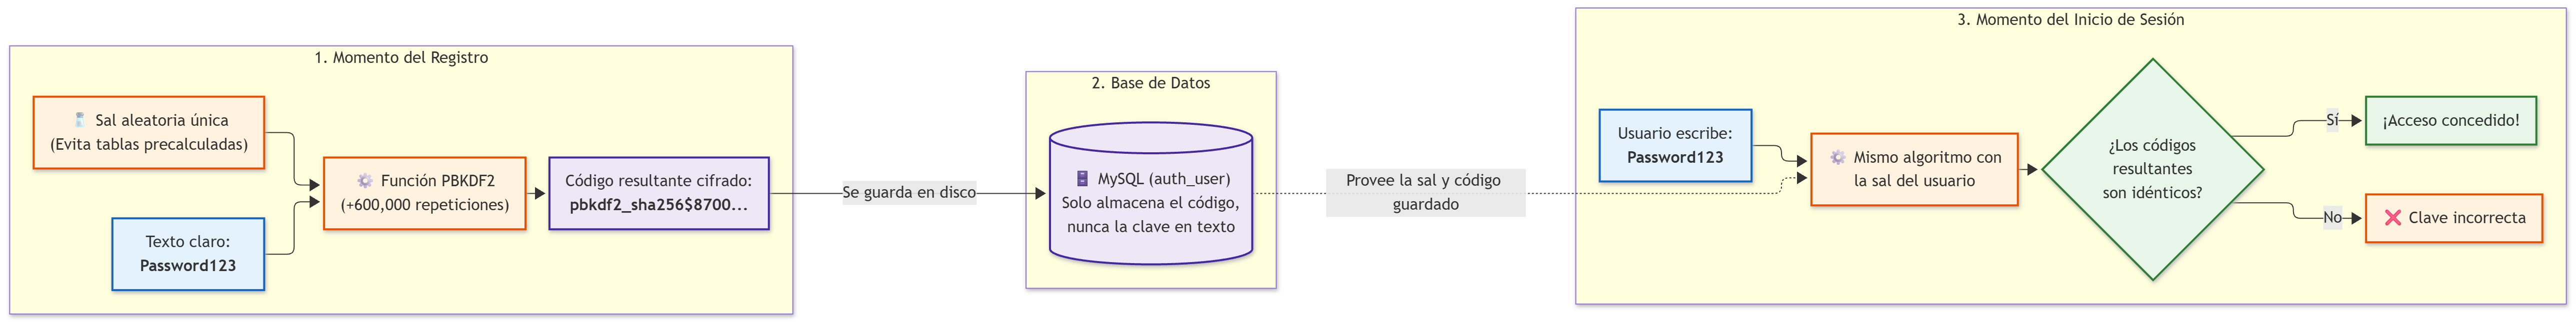
\includegraphics[width=\linewidth]{assets/seguridad/seguridad_contraseña.png}
    \caption{Proceso de protección de contraseñas mediante función Hash, sal aleatoria y comparación en el inicio de sesión.}
    \label{fig:seguridad_contrasena}
\end{figure}

\begin{itemize}
    \item \textbf{1. Momento del Registro:} Cuando el usuario crea su cuenta, el sistema toma su contraseña y le agrega un código secreto inventado al azar llamado ``sal'' (\textit{salt}). Esta mezcla entra a un triturador matemático que repite cálculos más de 600,000 veces. El resultado es un código revuelto único (por ejemplo: \texttt{pbkdf2\_sha256\$8700...}). La sal garantiza que, aunque dos alumnos elijan exactamente la misma contraseña, sus códigos guardados en la base de datos sean completamente distintos, evitando que se puedan adivinar usando listas de internet.
    \item \textbf{2. Guardado en Base de Datos:} En la tabla \texttt{auth\_user} de MySQL solo se almacena ese código largo junto con la sal; la contraseña original se olvida para siempre de la memoria.
    \item \textbf{3. Momento del Inicio de Sesión:} Cuando la persona regresa e intenta entrar, escribe su contraseña. El sistema no intenta descifrar el código que tenía guardado (porque es matemáticamente imposible revertirlo); en su lugar, toma la palabra recién escrita, le aplica la misma sal y el mismo cálculo, y compara los dos códigos resultantes. Si ambos códigos son idénticos, significa que la contraseña fue correcta y le abre la puerta al usuario; si son diferentes, le niega el paso.
\end{itemize}

\subsection{Validación Oficial de Asesores para Prevenir Cuentas Falsas}
\label{subsec:seguridad_validacion_docente}

En el Caso de Uso 1 (CU01), se debe asegurar que nadie pueda registrarse libremente fingiendo ser un profesor asesor para revisar o aprobar tesis sin autorización de la escuela. Para evitar este problema, el sistema cuenta con un circuito de aprobación supervisado por la coordinación académica.

En la Figura~\ref{fig:seguridad_asesor} se muestra el camino que sigue una cuenta de profesor antes de poder usarse:

\begin{figure}[H]
    \centering
    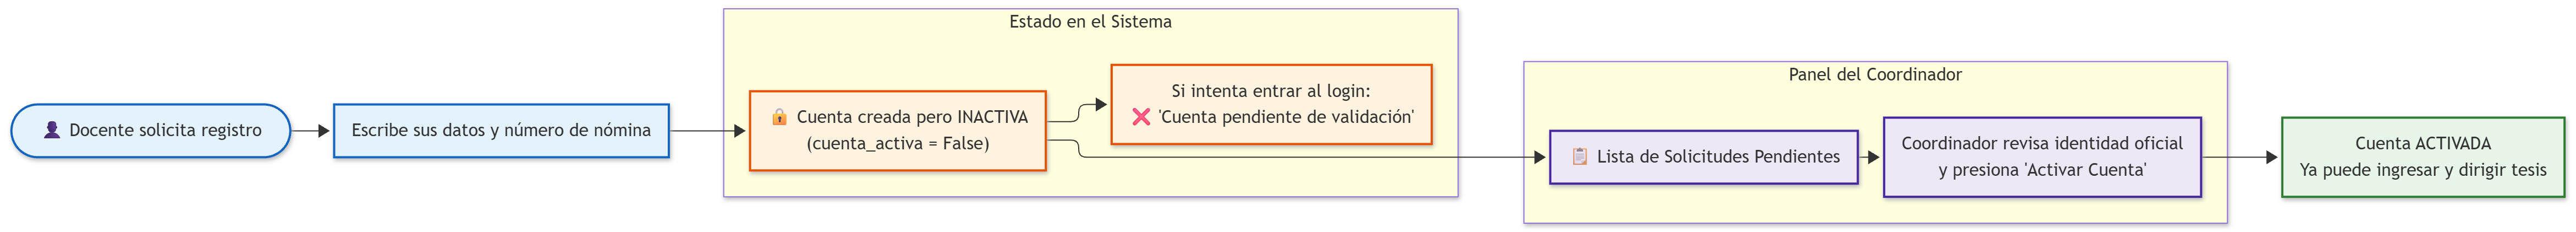
\includegraphics[width=\linewidth]{assets/seguridad/seguridad_asesor.png}
    \caption{Flujo de registro y activación supervisada para profesores asesores.}
    \label{fig:seguridad_asesor}
\end{figure}

\begin{enumerate}
    \item \textbf{Solicitud de registro:} El profesor llena el formulario con sus datos personales, su correo institucional y su número de nómina oficial.
    \item \textbf{Cuenta bloqueada por defecto:} El sistema crea el usuario pero le asigna automáticamente la casilla \texttt{cuenta\_activa = False}. Si el docente intenta iniciar sesión inmediatamente, la página le impide el acceso mostrando un aviso en color rojo que dice: ``Cuenta pendiente de validación''.
    \item \textbf{Revisión y activación escolar:} La solicitud aparece dentro del panel privado del coordinador. La coordinación revisa en las listas oficiales de la facultad que la persona sea un maestro en activo; una vez verificado, presiona el botón ``Activar Cuenta''. A partir de ese momento, la cuenta cambia a activa y el profesor ya puede entrar a la página a revisar borradores y levantar minutas.
\end{enumerate}

\subsection{Inspección Binaria de Archivos PDF en validators.py (Soporte al CU02)}
\label{subsec:seguridad_pdf_filtros}

En el Caso de Uso 2 (CU02), los estudiantes suben archivos digitales con sus borradores de tesis. La subida de archivos es uno de los puntos más delicados en una página web, porque un atacante podría intentar cambiarle el nombre a un programa con virus (por ejemplo, renombrar un archivo dañino de \texttt{virus.exe} a \texttt{tesis.pdf}) para engañar a la plataforma y ejecutarlo en el servidor.

Para impedir cualquier engaño, el archivo de validación \texttt{validators.py} somete cada entrega a un embudo de cuatro filtros consecutivos, tal como se ilustra en la Figura~\ref{fig:seguridad_pdf_estructura}:

\begin{figure}[H]
    \centering
    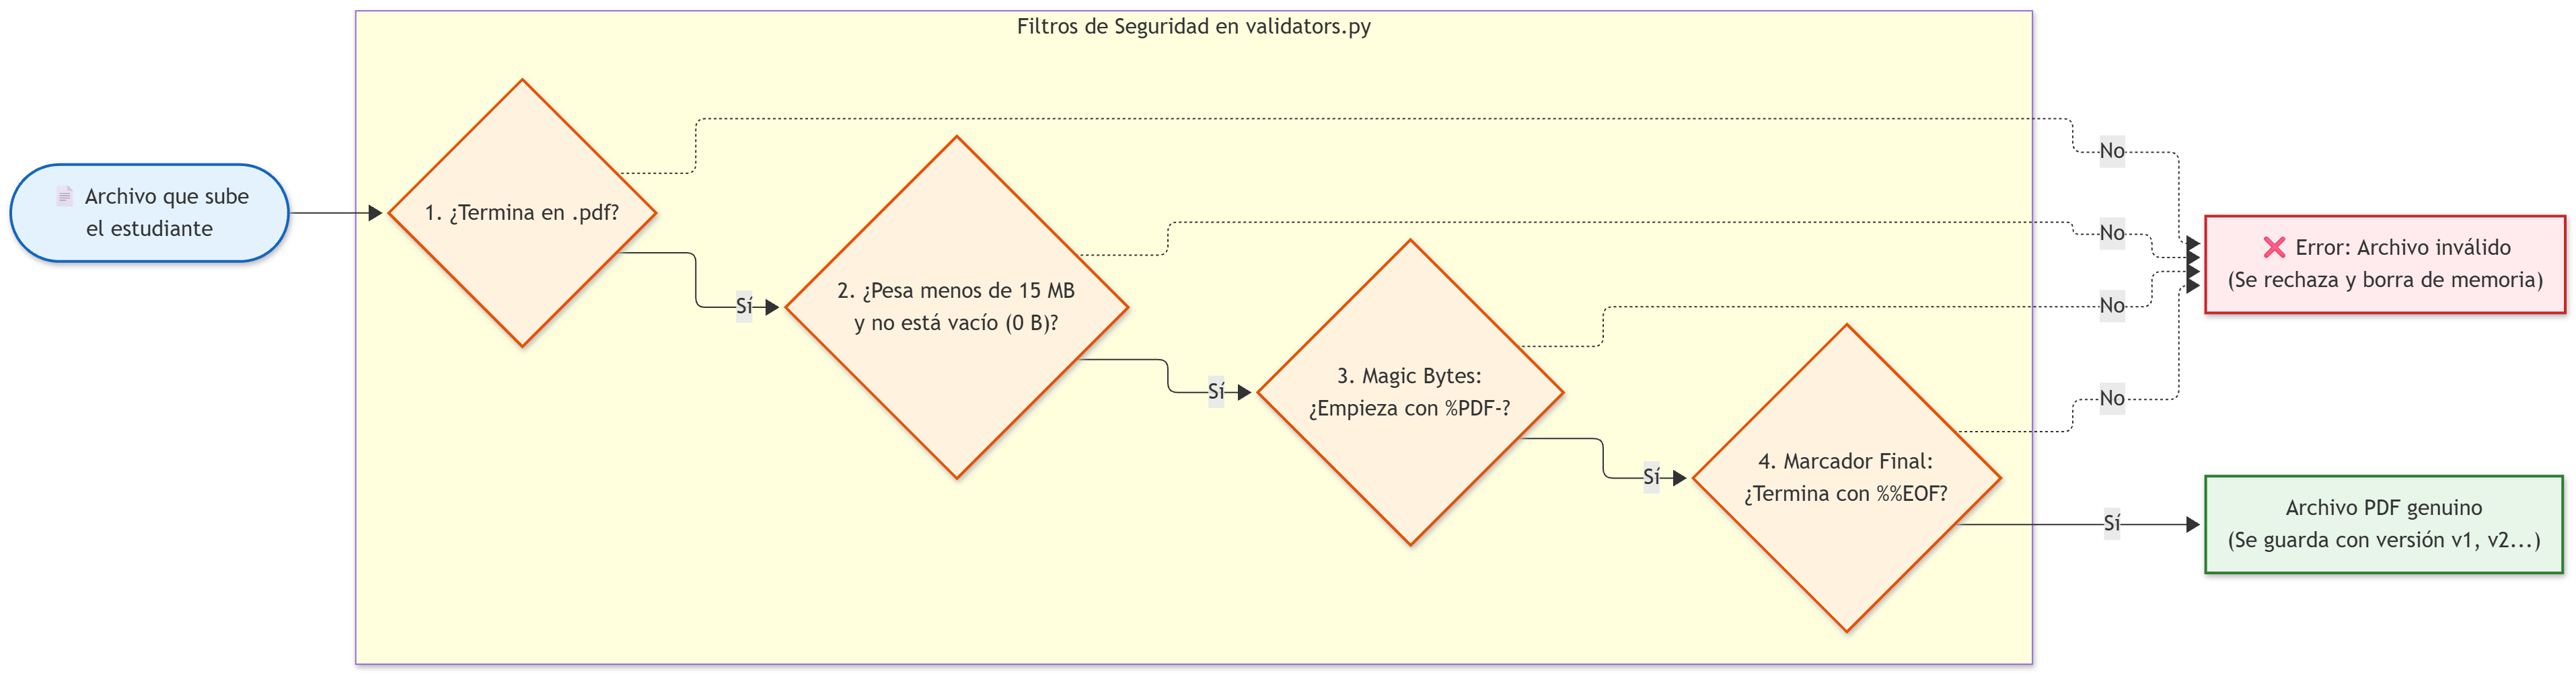
\includegraphics[width=\linewidth]{assets/seguridad/seguridad_pdf_estructura.png}
    \caption{Embudo de validación e inspección binaria de archivos en \texttt{validators.py}.}
    \label{fig:seguridad_pdf_estructura}
\end{figure}

\begin{itemize}
    \item \textbf{1. Revisión de extensión:} Comprueba que el nombre termine formalmente con las letras \texttt{.pdf}. Si termina en \texttt{.docx}, \texttt{.zip} o cualquier otra cosa, se descarta inmediatamente.
    \item \textbf{2. Control de peso y tamaño:} Verifica que el archivo no esté vacío (0 Bytes) y que no supere el límite permitido de 15 Megabytes, cuidando que el disco duro del servidor no se llene con archivos innecesariamente pesados.
    \item \textbf{3. Inspección de Magic Bytes (\%PDF-):} El sistema no se conforma con el nombre visible; abre el archivo en código binario y lee sus primeros caracteres en el disco. Todos los documentos PDF auténticos en el mundo comienzan obligatoriamente con la firma \texttt{\%PDF-}. Si un atacante solo le cambió el nombre a un ejecutable, el sistema se da cuenta al instante de que por dentro no es un PDF y lo borra de la memoria.
    \item \textbf{4. Marcador de cierre (\%\%EOF):} Por último, la función viaja al final del archivo para verificar que concluya con la etiqueta estándar \texttt{\%\%EOF} (\textit{End of File}). Esto garantiza que el borrador no esté roto, corrupto o incompleto por fallas en la conexión de internet del estudiante.
\end{itemize}

Únicamente los documentos que aprueban los cuatro filtros son recibidos por el sistema para asignarle su número consecutivo de versión ($v_1, v_2, \dots$).

\subsection{Interacción en el Tiempo del Guardado Seguro (Diagrama de Secuencia)}
\label{subsec:seguridad_secuencia_tiempo}

Para entender con claridad el orden cronológico en el que interactúan todas las partes de la plataforma al momento de entregar un borrador, en la Figura~\ref{fig:seguridad_pdf_tiempo} se presenta un diagrama de secuencia en el tiempo. En este esquema participan cuatro elementos: el \textbf{Alumno}, la \textbf{Página Web (Django)}, la \textbf{Base de Datos (MySQL)} y la \textbf{Carpeta de Archivos en Disco}.

\begin{figure}[H]
    \centering
    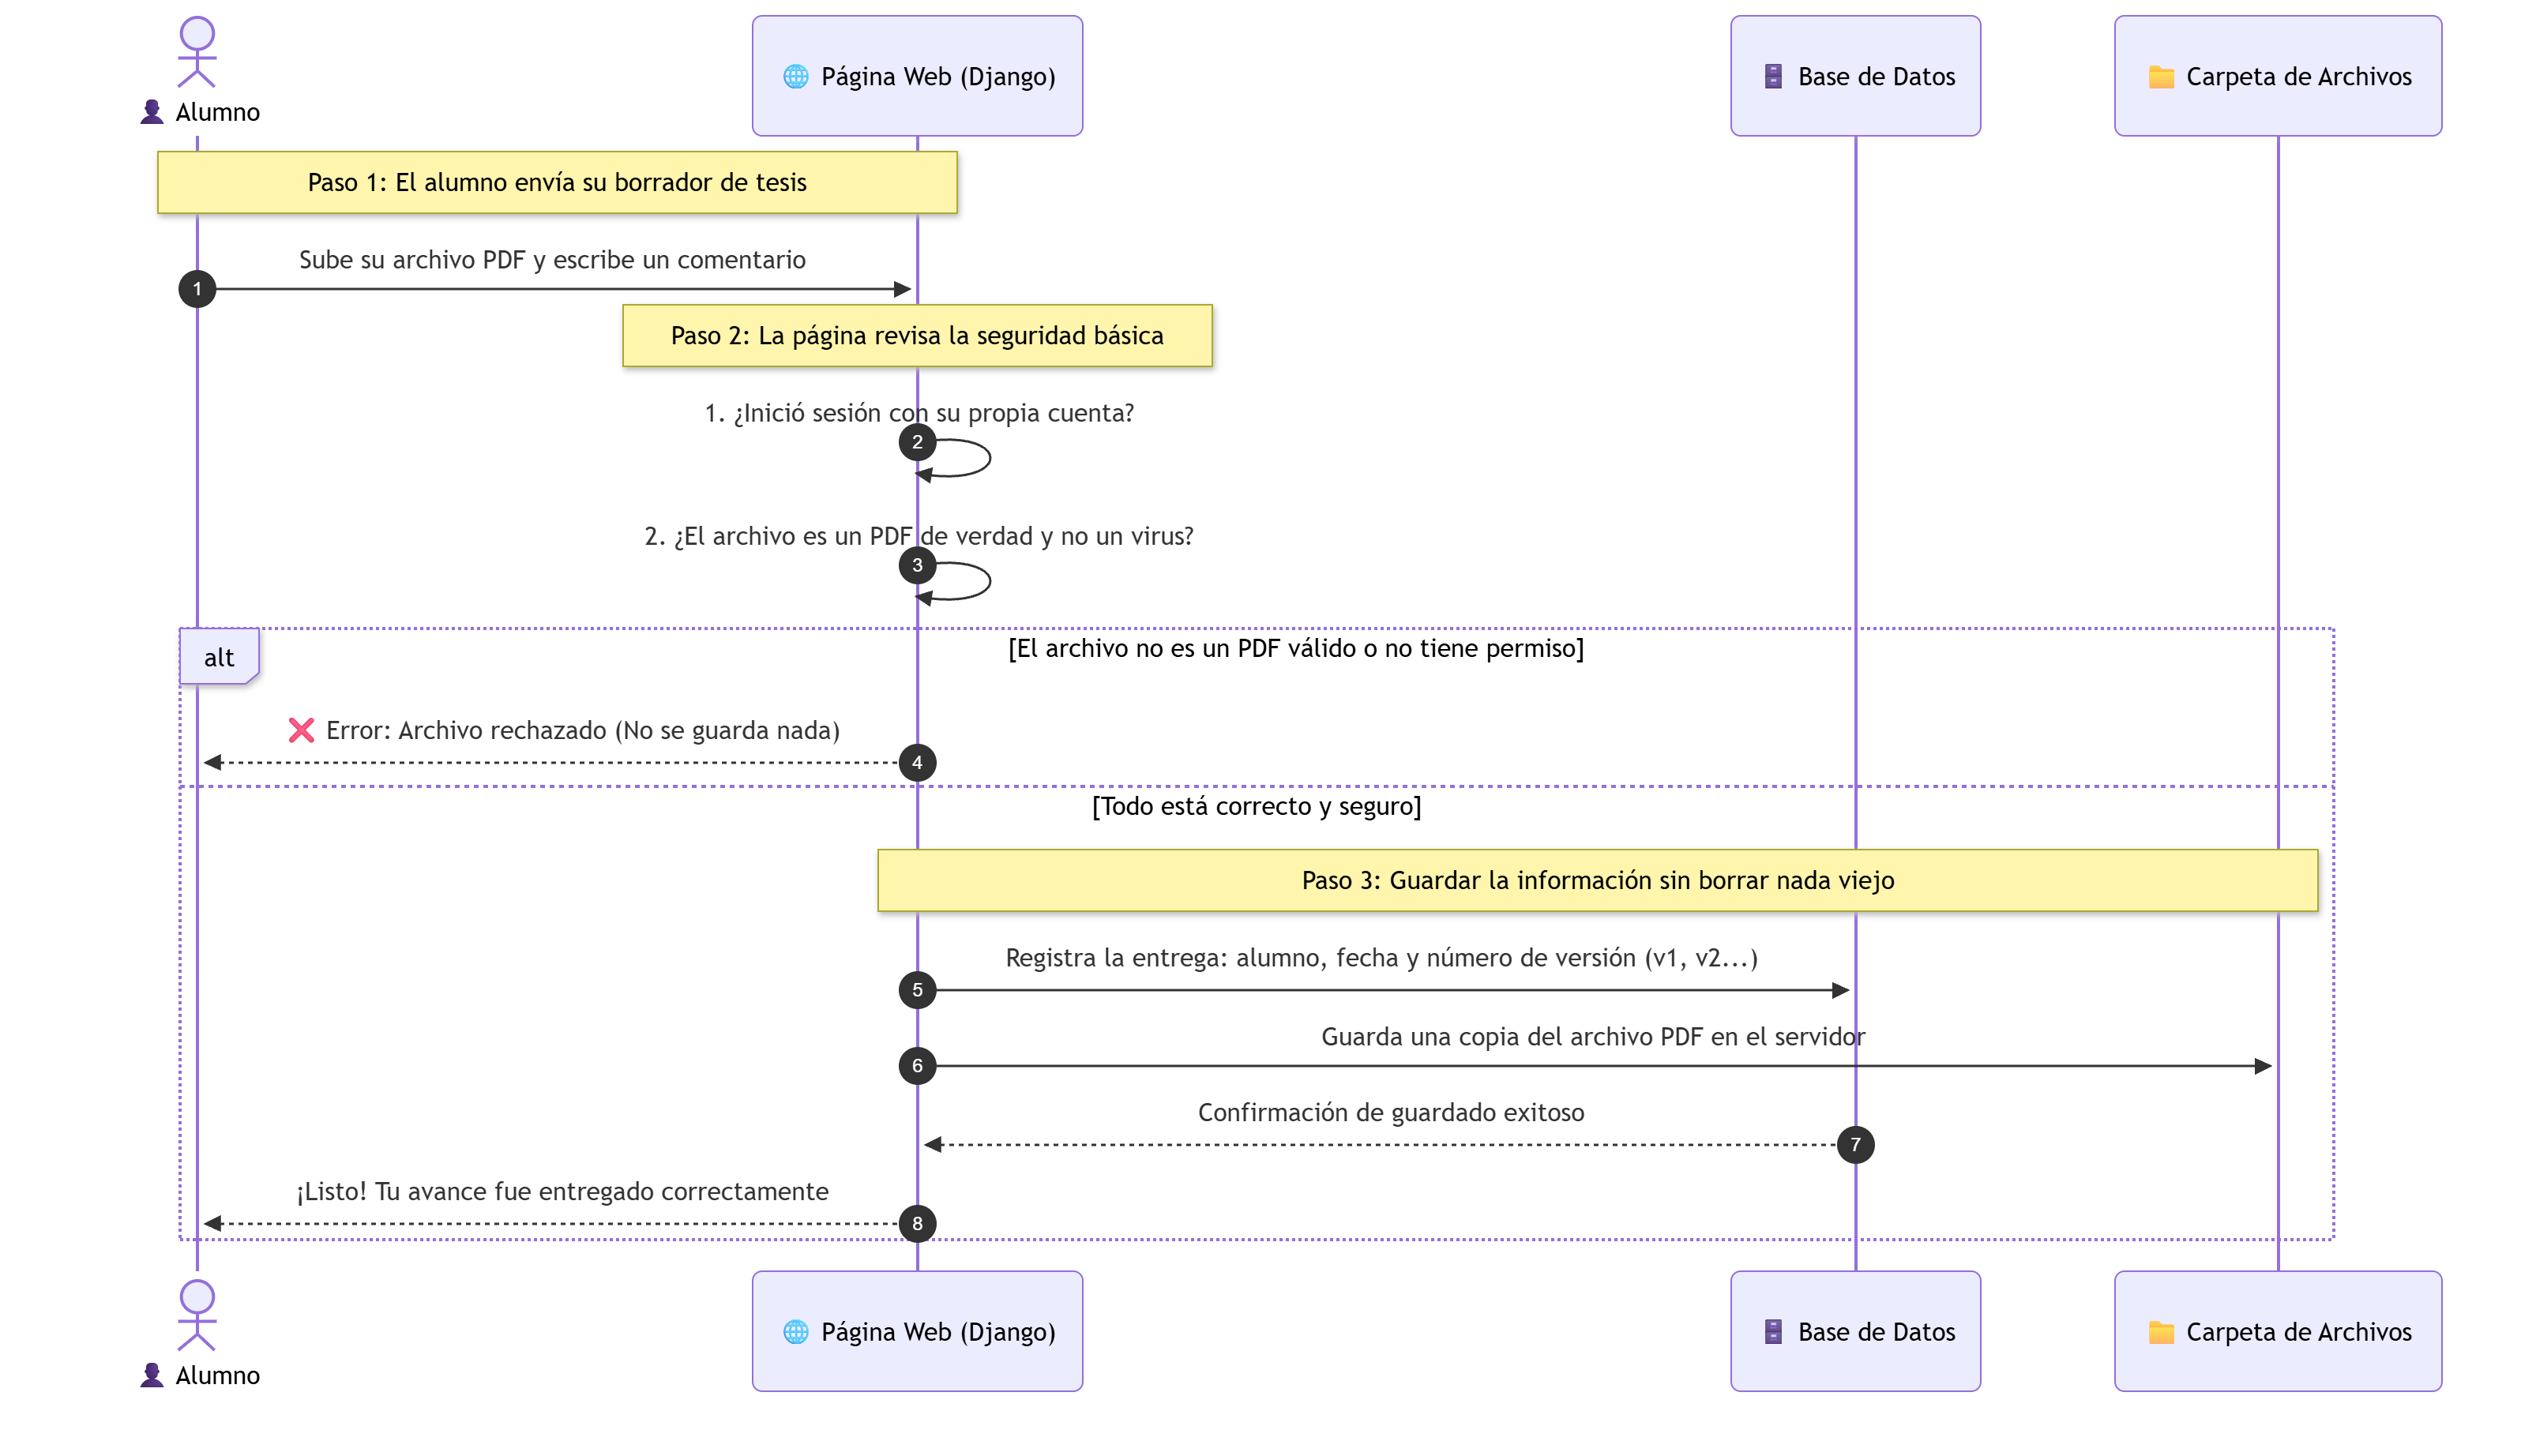
\includegraphics[width=\linewidth]{assets/seguridad/seguridad_pdf_tiempo.png}
    \caption{Diagrama de secuencia con las etapas cronológicas de revisión y guardado de un avance.}
    \label{fig:seguridad_pdf_tiempo}
\end{figure}

El proceso transcurre en tres grandes momentos enumerados del 1 al 8:

\begin{enumerate}
    \item \textbf{Paso 1: Envío del avance (Flecha 1):} El estudiante selecciona el archivo PDF en su computadora, escribe una nota de entrega y presiona el botón de subida.
    \item \textbf{Paso 2: Inspección previa (Flechas 2 y 3):} La página web detiene la entrega por unos milisegundos para verificar dos cosas: primero, que el usuario tenga su propia sesión iniciada (evitando accesos indebidos o suplantaciones), y segundo, que el archivo sea un PDF íntegro pasando por el embudo de validación antes mencionado.
    \item \textbf{Filtro de decisión (Bloque \textit{alt}):}
    \begin{itemize}
        \item \textbf{Camino de rechazo (Flecha 4):} Si el archivo venía dañado, pesaba demasiado o no era un PDF genuino, la página le avisa al alumno con un mensaje de error y el proceso termina ahí; la base de datos ni el disco se tocan.
        \item \textbf{Camino exitoso (Flechas 5 a 8):} Si la revisión fue positiva, la página le ordena a MySQL registrar la entrega con el alumno, la fecha y el número de versión correlativo (v1, v2...); copia físicamente el PDF a la carpeta protegida de medios; la base de datos confirma el guardado; y finalmente la pantalla muestra el aviso en verde confirmando que la entrega se completó exitosamente.
    \end{itemize}
\end{enumerate}

\subsection{Consultas Parametrizadas y Prevención de Inyecciones SQL}
\label{subsec:seguridad_datos_arco}

Para completar el blindaje de la plataforma en la base de datos MySQL, el código del backend utiliza de manera obligatoria el mapeador objeto-relacional (ORM) de Django con consultas parametrizadas en todas las vistas. 

Esto significa que cuando un usuario busca una tesis o consulta una minuta, los parámetros ingresados se envían totalmente aislados de las instrucciones lógicas de la base de datos, impidiendo cualquier ataque de inyección SQL (SQLi). Asimismo, la cuenta de conexión del sistema opera bajo el principio de privilegio mínimo exclusivo sobre el esquema \texttt{tesina\_db}, garantizando que ningún usuario ajeno pueda consultar o alterar información externa al posgrado.